\section{Proposed Method}	
2D polygonal profile is decomposed  into sub-polygons. Sub polygons being simpler, make Midcurves creation more deterministic than getting the same from the whole profile.

\subsection{Decomposition}
Polygons come with different types of variations. They can be simple/self-intersecting, with/without holes, concave/convex etc. This work focuses on a special type, an elongated polygon for which Midcurves can be generated e.g. alphabets made using Ribbon-like shapes. For this paper, more focus is given on profiles with constant thickness with test cases based on English alphabets. 

Important points to note are \cite{Bayazit}:
\begin{enumerate}
\item A polygon can be broken into convex regions by eliminating all reflex vertices.
\item A reflex vertex can only be removed if the diagonal connecting to it is within the range given by extending its neighboring edges; otherwise, its angle is only reduced.
\end{enumerate}

\subsubsection{Preliminaries}

\begin{list}{}{}
\item {\bf Polygon}: A polygon $P$ of $n$ vertices is defined as 

$P = \{P_0,P_1,...,P_{n-1}\}$

where, the vertices are in counter clockwise (ccw) order. Polygon $P$ can also be defined in terms of a set of connected edges as  

$P = \{\overline{P_0 P_1},\overline{P_1 P_2}...,\overline{P_{n-1} P_0}\}$

In case of shapes which have non-linear elements, they are faceted and brought in terms of connected lines.

\item {\bf Simple}: A polygon is simple if none of the edges intersect other edges anywhere else other than the shared endpoints of adjacent edges.
\begin{displaymath}
\forall \quad \overline{P_i P_j}, \overline{P_k P_l} \in P, \left\{ 
  \begin{array}{l l}
     \overline{P_i P_j} \cap \overline{P_k P_l} = \phi , j \neq k\\
     \overline{P_i P_j} \cap \overline{P_k P_l} = P_k  , j = k
  \end{array} \right.
\end{displaymath}

\item {\bf Diagonal}: $\overline{P_i P_k}$ is a {\em diagonal} of $P$.  In other words, a {\em diagonal} is just a line segment between two vertices that only touches the interior of the polygon.

\item {\bf Area}: $Area$ formed by three vertices in order ($ P_{j-1}, P_j,  P_{j+1}$) or two consecutive {\em edges} ($ \overline{P_{j-1} P_j} \cap \overline{P_j P_{j+1}}$ ) is a signed quantity which is given by
\begin{displaymath}
\begin{array}{l l}
Area = P_{j-1}.X ( P_j.Y - P_{j+1}.Y) + \\
P_j.X (P_{j+1}.Y -  P_{j-1}.Y) + \\
P_{j+1}.X ( P_{j-1}.Y - P_j.Y) 
 \end{array} 
\end{displaymath}

\item {\bf Left}: $P_{j+1}$ is {\em Left} of $ \overline{P_{j-1} P_j}$ if $Area( P_{j-1}, P_j,  P_{j+1}) > 0$ 

\item {\bf Right}: $P_{j+1}$ is {\em Right} of $ \overline{P_{j-1} P_j}$ if $Area( P_{j-1}, P_j,  P_{j+1}) < 0$ 

\item {\bf Collinear}: $P_{j+1}$ is {\em Collinear} with $ \overline{P_{j-1} P_j}$ if $Area( P_{j-1}, P_j,  P_{j+1}) = 0$ 

\item {\bf Reflex}: Let  $ P_{j-1}, P_j,  P_{j+1} \in P $ , if the interior $\angle P_{j-1}, P_j,  P_{j+1}$ is greater than $\pi$  then $P_j$  is a concave or {\em reflex} vertex. $Area < 0$

\item {\bf Intersect}: For  $\overline{P_i P_j}$ to intersect $\overline{P_k P_l}$, either of $P_k, P_l$ should be on {\em Left} of  $\overline{P_i P_j}$ and the other vertex should be on {\em Right}. Intersection could be of {\em Line} type where extended intersection can be calculated or of {\em Segment} type where only internal intersections are returned.

\item {\bf Visibility/Can-See}: $P_k$ is visible from $P_i$ if $\overline{P_i P_k}$ is a {\em diagonal} of $P$. 

\end{list}

\subsubsection{Steps}
Let $P$ be a simple polygon.  The Partitioning of $P$ is defined by the decomposition of $P$ into partitions of non-overlapping sub-polygons by adding internal {\em diagonals} between vertices  $P_i$ or by adding new (Steiner) vertices on {\em edges} $\overline{P_i P_j}$.

%\begin{tabular}[h]{@{}p{5cm}  p{3cm}@{}}
\begin{list}{}{}

%------------------------------------------------------------------------------------------------------------------------------------
\item 
Go through all the vertices of the polygon one by one in counter-clockwise manner. Current vertex is called $P_i$ %&

\raisebox{-.9\height}{\includegraphics[scale=0.29]{..//Common/images/polydecomp_traverse.png} }%\\

%------------------------------------------------------------------------------------------------------------------------------------
\item 
Check if $P_i$ is a Reflex vertex $R$  %&



\raisebox{-.9\height}{\includegraphics[scale=0.3]{..//Common/images/polydecomp_reflex.png} }%\\

%------------------------------------------------------------------------------------------------------------------------------------
\item 
Extend lines incident at $P_i$ (the line coming into $P_i$ and going out of $P_i$ ) till they intersect remaining of the Polygon, say at $Q_1$ and $Q_2$. Contour within $Q_1$ and $Q_2$ is called $Range$ %&

\raisebox{-.9\height}{\includegraphics[scale=0.3]{..//Common/images/polydecomp_range.png} }%\\

%------------------------------------------------------------------------------------------------------------------------------------
\item 
If there are no $P_i$s within the $Range$, create a new one at the middle on the contour. This newly created point  $Q_m$ is called Steiner point.  $RQ_m$ is the partition-chord to divide the polygon %&

\raisebox{-.9\height}{\includegraphics[scale=0.37]{..//Common/images/polydecomp_mid.png} }%\\

%------------------------------------------------------------------------------------------------------------------------------------
\item 
If there are few vertices within the $Range$, choose best one based on following priorities.
\begin{enumerate}
\item Highest : Closest Reflex 
\item Medium : Reflex 
\item Low : Closest 
\end{enumerate} 
%&

\raisebox{-.9\height}{\includegraphics[scale=0.37]{..//Common/images/polydecomp_choice.png} }%\\

%------------------------------------------------------------------------------------------------------------------------------------
\item 
Once vertex is chosen, say, $Q_i$, create partition chord $RQ_i$ and divide the  polygon.% &

\raisebox{-.9\height}{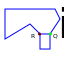
\includegraphics[scale=0.37]{..//Common/images/polydecomp_divide.png} } %\\


%\end{tabular}

%------------------------------------------------------------------------------------------------------------------------------------
\item 
Send individual sub-polygons to the same process recursively till there are no reflex vertices left. 

\end{list}



\begin{algorithm}
	\caption{Polygon Decomposition}
	\label{alg1}
	\begin{algorithmic}
		\REQUIRE 2D Planar polygon represented by list of vertices
		\ENSURE Vertices in counter-clockwise direction

		\WHILE{End of vertices list has  not reached}
			\STATE Get the current vertex.
			\IF {current vertex is a Reflex vertex $R$}           
				\STATE Extend  the  edges incident at $R$ until they hit an edge

				\IF {Extension line and Polygon side are collinear} 				
					\STATE Find closest point which is not internal to the extension line
				\ENDIF

				\IF {there are no vertices to connect to} 				
					\STATE choose a point in the middle
				\ELSE
					\STATE Find vertex to connect to
					\STATE Find best vertex $B$ within the range, to form the partitioning chord
					\STATE Make sure $B$ is visible from $R$
				\ENDIF
			\ENDIF
		\ENDWHILE
		\STATE  Split the polygon at the cutting chord (line $RB$)
	\end{algorithmic}
\end{algorithm}

\subsection{Improvements over Bayazit's algorithm}

{\bf Algorithm \ref{alg1}} improves upon the Beyazit's algorithm \cite{Bayazit} in terms of expanding search to even include extreme vertices in the range thereby giving minimal and elongated partitions. Midcurves are typically for thin-elongated shapes. This improvement results in the sub-polygons of necessary shape characteristics.

\begin{tabular}[h]{@{} p{0.55\linewidth}  p{0.3\linewidth}@{}}

 If any of the incoming edges was hitting end points of test line or was collinear, it was getting ignored in the existing algorithm \cite{Bayazit} and then the next closet vertex was getting chosen.  &

\raisebox{-.9\height}{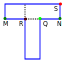
\includegraphics[scale=0.29]{..//Common/images/polydecomp_mine.png} }\\
\end{tabular}
 It has been avoided in the improved algorithm which can be clearly seen in the results shown in Table {\bf Table \ref{PartitionComparision}}.




{\bf Table \ref{PartitionComparision}} demonstrates improvements over Beyzit's \cite{Bayazit} algorithm with examples.  



\begin{table}[!h]
\caption{Improvement Over current partitioning algorithm}
\begin{tabular}[h]{@{}p{0.2\linewidth} p{0.2\linewidth}  p{0.2\linewidth} p{0.2\linewidth} @{}}
\toprule

{\bf Type } & {\bf Shape } & {\bf Earlier} & {\bf Proposed}\\
\midrule
%------------------------------------------------------------------------------------------------------------------------------------
T: Extra-Longer split was unnecessary &
\raisebox{-.9\height}{\includegraphics[scale=0.17]{..//Common/images/Ts.png}} &
\raisebox{-.9\height}{\includegraphics[scale=0.17]{..//Common/images/Tb.png}}&
\raisebox{-.9\height}{\includegraphics[scale=0.17]{..//Common/images/Tp.png}} \\


%------------------------------------------------------------------------------------------------------------------------------------
Plus : Extra-Longer splits unnecessary &
\raisebox{-.9\height}{\includegraphics[scale=0.17]{..//Common/images/Pluss.png}} &
\raisebox{-.9\height}{\includegraphics[scale=0.17]{..//Common/images/Plusb.png}}&
\raisebox{-.9\height}{\includegraphics[scale=0.17]{..//Common/images/Plusp.png}} \\


%------------------------------------------------------------------------------------------------------------------------------------
Star : Splitting was not at the closest Reflex &
\raisebox{-.9\height}{\includegraphics[scale=0.17]{..//Common/images/Stars.png}} &
\raisebox{-.9\height}{\includegraphics[scale=0.17]{..//Common/images/Starb.png}}&
\raisebox{-.9\height}{\includegraphics[scale=0.17]{..//Common/images/Starp.png}} \\

\bottomrule
\end{tabular}
\label{PartitionComparision}
\end{table}

The resulting sub-polygons are sent for creating connected midcurves.


\subsection{Midcurves Generation}

Decomposition helped getting the sub-polygons which are of primitive shapes and which are easier for Midcurves creation compared to original-whole shape. 

\begin{tabular}[h]{@{}p{0.6\linewidth} p{0.3\linewidth}@{}}

%\begin{itemize}
%------------------------------------------------------------------------------------------------------------------------------------
Partitioning: Decompose Polygons into  sub-polygons of primitive shapes using {\bf Algorithm \ref{alg1}}. Each additional edge inserted during the decomposition is called as 'chord'. &

\raisebox{-.9\height}{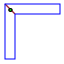
\includegraphics[scale=1.2]{..//Common/images/midcurve_polydecomp.pdf} }\\


%------------------------------------------------------------------------------------------------------------------------------------
Generate Midcurves for individual polygons taking chords into consideration. 'Thinness' is an important criterion in choosing midcurves for the individual shape. Midcurves are generated along longer-length and not across shorter width. &
\raisebox{-.9\height}{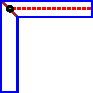
\includegraphics[scale=1.2]{..//Common/images/midcurve_polymid.pdf} }\\


%------------------------------------------------------------------------------------------------------------------------------------
In shapes like 'L' midcurves from both sub-polygons, across the chord, join together at a point, naturally. But in case of shapes like 'T', the horizontal midcurve does not connect with the common chord. In this case one of the midcurves needs to be extended to join the other. &

\raisebox{-.9\height}{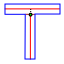
\includegraphics[scale=1.2]{..//Common/images/midcurve_extend.pdf} }\\

%\end{itemize}
\end{tabular}
%\vspace{.1cm}

Each such shape can create its own Midcurves based on number of sides and also where the cutting-chords lie on this individual shape. Tables \ref{Configurationst}, \ref{Configurationsp} have more details. Chord is a common interface-boundary shared between two sub-polygons. Each chord will have two sides owned by two different sub-polygons. Each sub-polygon needs to look at it's own shape, slenderness and decide own Midcurve.

\begin{table}[!h]
\caption{Triangle cases of Midcurve configuration}
\begin{tabular}[h]{@{}p{0.16\linewidth}@{} p{0.18\linewidth} @{}p{0.36\linewidth} p{0.15\linewidth}@{}} \toprule
{\bf Shape } & {\bf Chords }  & {\bf Rule} & {\bf Diagram}\\
\midrule

%------------------------------------------------------------------------------------------------------------------------------------
Triangle &
None&
No Midcurve &
\raisebox{-.9\height}{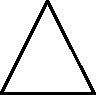
\includegraphics[scale=0.9]{..//Common/images/mids_t0.pdf} }\\

%------------------------------------------------------------------------------------------------------------------------------------
&
One &
Join Opposite vertex &
\raisebox{-.9\height}{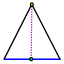
\includegraphics[scale=0.9]{..//Common/images/mids_t1.pdf} }\\


%------------------------------------------------------------------------------------------------------------------------------------
&
Two &
Join midpoints &
\raisebox{-.9\height}{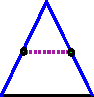
\includegraphics[scale=0.9]{..//Common/images/mids_t2.pdf} }\\

%------------------------------------------------------------------------------------------------------------------------------------
&
Three &
Join to centroid &
\raisebox{-.9\height}{\includegraphics[scale=0.9]{..//Common/images/mids_t3.pdf} }\\

\bottomrule

\end{tabular}
\label{Configurationst}
\end{table}

\begin{table}[!h]
\caption{Polygon cases of Midcurve configuration}
\begin{tabular}[h]{@{}p{0.13\linewidth} p{0.18\linewidth}  p{0.35\linewidth}  p{0.15\linewidth}@{}} \toprule

{\bf Shape } & {\bf Chords }  & {\bf Rule} & {\bf Diagram}\\
\midrule
%------------------------------------------------------------------------------------------------------------------------------------
Quad &
None&
Find shortest side and create Midcurve in the direction average of both the adjacent sides &
\raisebox{-.9\height}{\includegraphics[scale=0.9]{..//Common/images/mids_q0.pdf} }\\

%------------------------------------------------------------------------------------------------------------------------------------
&
One (Shorter) &
Create Midcurve in the direction average of both the adjacent sides &
\raisebox{-.9\height}{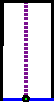
\includegraphics[scale=0.9]{..//Common/images/mids_q1s.pdf} }\\


%------------------------------------------------------------------------------------------------------------------------------------
&
One (Longer)&
None &
\raisebox{-.9\height}{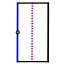
\includegraphics[scale=0.9]{..//Common/images/mids_q1l.pdf} }\\


%------------------------------------------------------------------------------------------------------------------------------------
&
Two (Opposite)&
Join midpoints &
\raisebox{-.9\height}{\includegraphics[scale=0.9]{..//Common/images/mids_q2o.pdf} }\\


%------------------------------------------------------------------------------------------------------------------------------------
&
Two (Adjacent) &
Ignore the chord on longer side and use one-chord rule &
\raisebox{-.9\height}{\includegraphics[scale=0.9]{..//Common/images/mids_q2a.pdf} }\\


%------------------------------------------------------------------------------------------------------------------------------------
&
Three &
Join to centroid &
\raisebox{-.9\height}{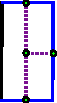
\includegraphics[scale=0.9]{..//Common/images/mids_q3.pdf} }\\


%------------------------------------------------------------------------------------------------------------------------------------
&
Four &
Join to centroid &
\raisebox{-.9\height}{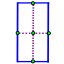
\includegraphics[scale=0.9]{..//Common/images/mids_q4.pdf} }\\

%\end{tabular}
%\label{Configurationsq}
%\end{table}
%
%\begin{table}[!h]
%\caption{Polygon cases of Midcurve configuration}
%\begin{tabular}[h]{|p{1cm} | p{1cm} | p{3cm} | p{1.2cm}|}
%\hline
%{\bf Shape } & {\bf Chords }  & {\bf Rule} & {\bf Diagram}\\
%\hline

%------------------------------------------------------------------------------------------------------------------------------------
Polygon &
None&
None &
\raisebox{-.9\height}{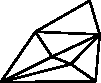
\includegraphics[scale=0.9]{..//Common/images/mids_p0.pdf} }\\

%------------------------------------------------------------------------------------------------------------------------------------
&
Any &
Join to centroid &
\raisebox{-.9\height}{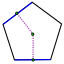
\includegraphics[scale=0.9]{..//Common/images/mids_pany.pdf} }\\
\bottomrule

\end{tabular}
\label{Configurationsp}
\end{table}



After creating individual Midcurves, they all may or may not join the chords. In case it does not join to any side of the chord, some extension has to be provided from other side of that chord. Chords are processed to ignore the ones which have partial overlap with the sub-polygon sides or are collinear. This method gives cleaner (without branches) and connected Midcurves compared to previously cited methods. Pseudo code for Midcurve generation process is presented in Algorithm \ref{alg2}.

\begin{algorithm}[!h]
	\caption{Midcurves Creation}
	\label{alg2}
	\begin{algorithmic}
		\REQUIRE List of partitioned 2D Planar polygons represented by list of vertices in counter-clockwise direction
		\STATE Find internal-common edges called chords
		\STATE Iterate over all polygons and create chords at Full or Partial overlap
		\WHILE{End of Polygons list has  not reached}
			\STATE Get the current polygon $P$
			\STATE Get chords which are part of $P$
			\STATE Look at various combinations-configurations due to Num Sides and Num Chords
			\STATE Generate Midcurves
			\STATE Assign Midcurves on relevant side of the chord
		\ENDWHILE
		\STATE Extend chords which are not connected with other neighboring chords
	\end{algorithmic}
\end{algorithm}


\section{Results}


Table \ref{MedialsPartition} briefly summarizes results of Decomposition and Midcurves creation for some sample polygons. Many examples shown here are of English alphabets as they present various ways of connectivity, have curves, holes and are easier to imagine and verify.

\begin{table}[!h]
\caption{Partitions-Medial Computation}
\begin{tabular}[h]{@{}p{0.24\linewidth} p{0.18\linewidth} p{0.18\linewidth} p{0.18\linewidth}@{}}
\toprule
{\bf Type } & {\bf Shape } & {\bf Partitions} & {\bf Midcurves}\\
\midrule
%------------------------------------------------------------------------------------------------------------------------------------
L: Midcurves on both sides of the chord, joined &
\raisebox{-.9\height}{\includegraphics[scale=0.15]{..//Common/images/Ls.png}} &
\raisebox{-.9\height}{\includegraphics[scale=0.15]{..//Common/images/Lp.png}}&
\raisebox{-.9\height}{\includegraphics[scale=0.15]{..//Common/images/Lm.png}} \\


%------------------------------------------------------------------------------------------------------------------------------------
T : Midcurve only on one side; need to extend to join &
\raisebox{-.9\height}{\includegraphics[scale=0.15]{..//Common/images/Ts.png}} &
\raisebox{-.9\height}{\includegraphics[scale=0.15]{..//Common/images/Tp.png}}&
\raisebox{-.9\height}{\includegraphics[scale=0.15]{..//Common/images/Tm.png}} \\


%------------------------------------------------------------------------------------------------------------------------------------
Plus : Midcurve only on either sides; need to extend to join &
\raisebox{-.9\height}{\includegraphics[scale=0.15]{..//Common/images/Pluss.png}} &
\raisebox{-.9\height}{\includegraphics[scale=0.15]{..//Common/images/Plusp.png}}&
\raisebox{-.9\height}{\includegraphics[scale=0.15]{..//Common/images/Plusm.png}} \\

%------------------------------------------------------------------------------------------------------------------------------------
Y : Collinear chord ignored; need to extend to join &
\raisebox{-.9\height}{\includegraphics[scale=0.15]{..//Common/images/Ys.png}} &
\raisebox{-.9\height}{\includegraphics[scale=0.15]{..//Common/images/Yp.png}}&
\raisebox{-.9\height}{\includegraphics[scale=0.15]{..//Common/images/Ym.png}} \\
\bottomrule

\end{tabular}
\label{MedialsPartition}
\end{table}

